\authoredSection{corny}{Toolchain}
Im Rahmen unseres Projekts wurde uns schnell klar, dass wir auf viele Tools angewiesen sein würden. So musste unser Quelltext versioniert, die grobe Struktur und Views festgehalten und Aufgabenpakete erstellt und koordiniert werden. Darüber hinaus war uns auch Design und Qualität wichtig. Auf unsere Erfahrungen in diesem Zusammenhang gehen wir im folgenden Abschnitt ein.

\subsection{Agiles Vorgehen im Projekt}
PivotalTracker + Scrum
\begin{figure}
	\centering
	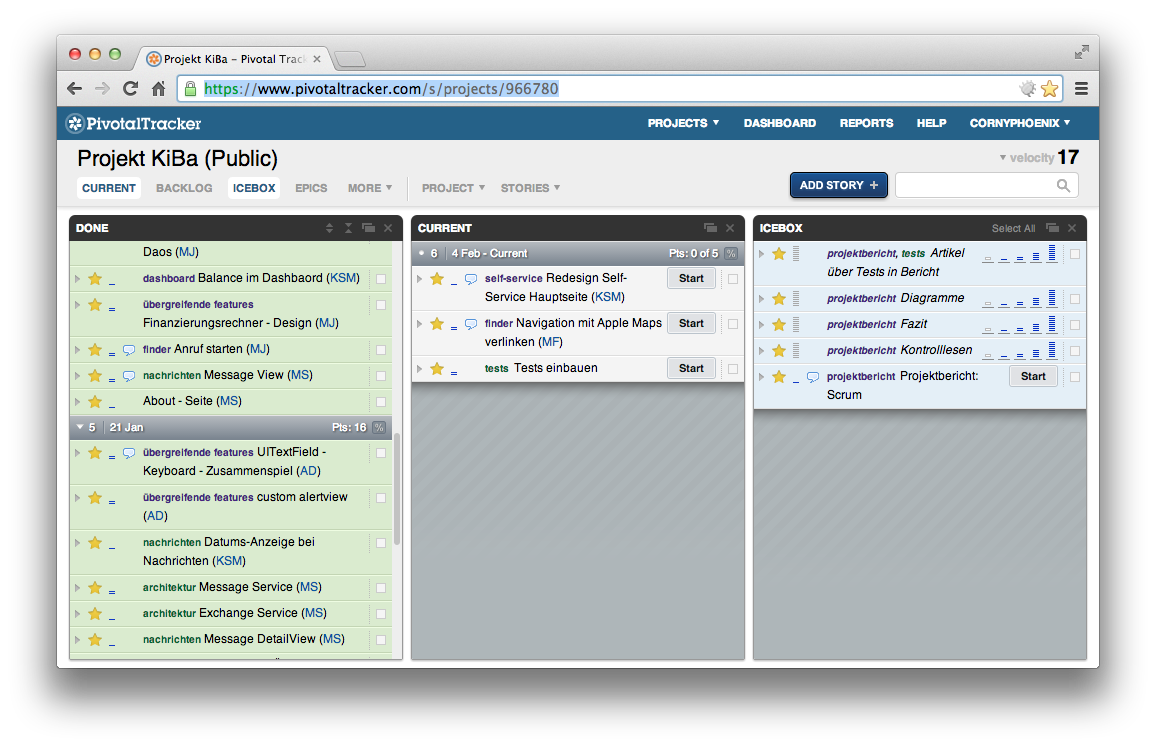
\includegraphics[scale=.3]{Pictures/TrackerStories}
	\label{fig:TrackerStories}
	\caption{Stories in PivotalTracker}
\end{figure}
\begin{figure}
	\centering
	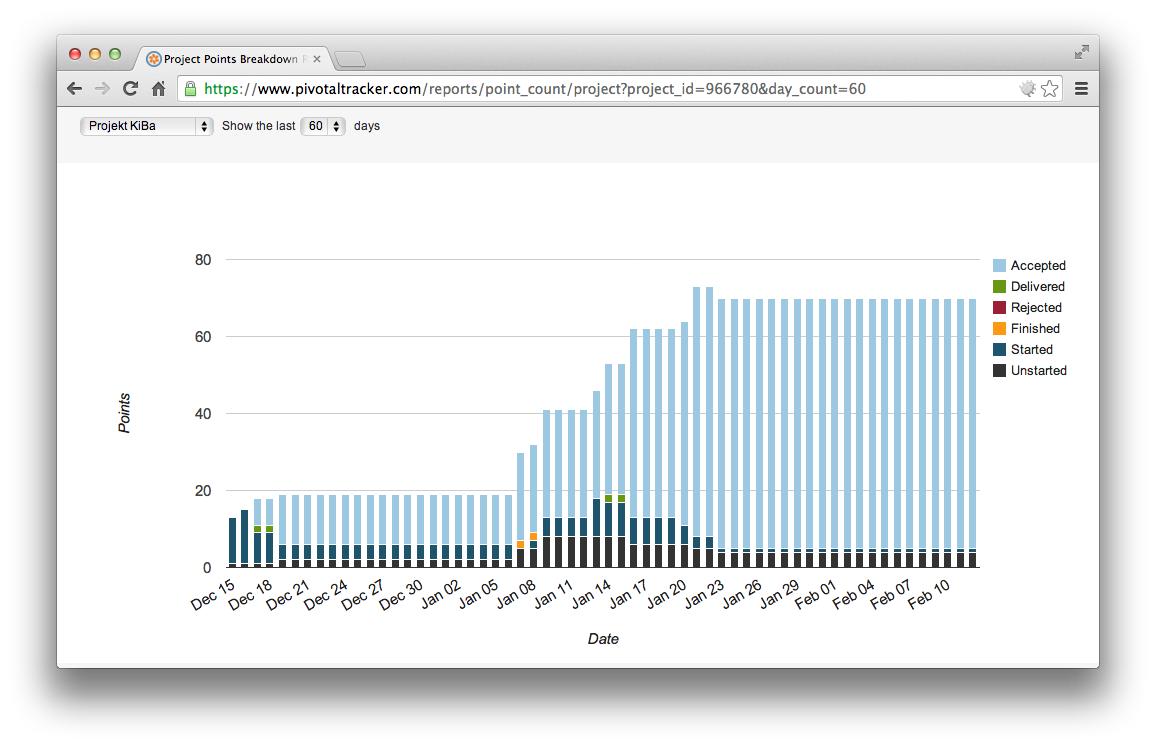
\includegraphics[scale=.3]{Pictures/TrackerBurndown}
	\label{fig:TrackerBurndown}
	\caption{Burndown-Chart in PivotalTracker}
\end{figure}

\subsection{Quelltextversionierung}
GitHub + Git
\begin{figure}
	\centering
	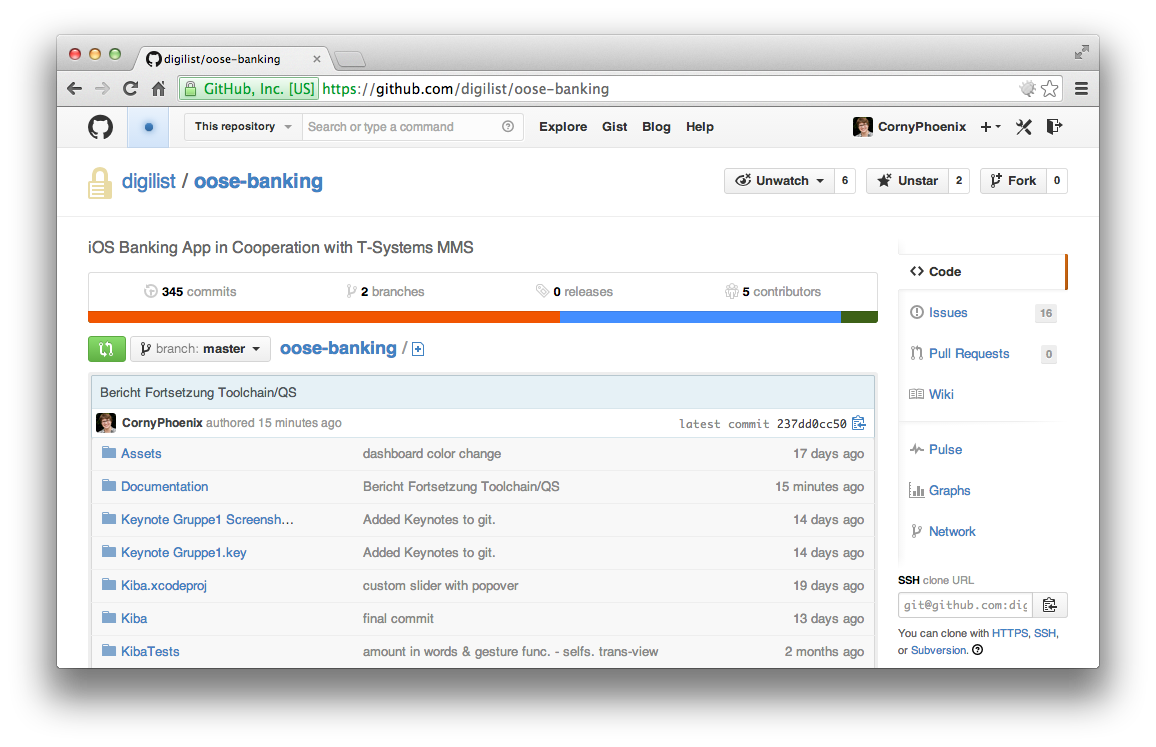
\includegraphics[scale=.3]{Pictures/GitHubOverview}
	\label{fig:GitHubOverview}
	\caption{Quelltext-Hosting bei GitHub}
\end{figure}
\begin{figure}
	\centering
	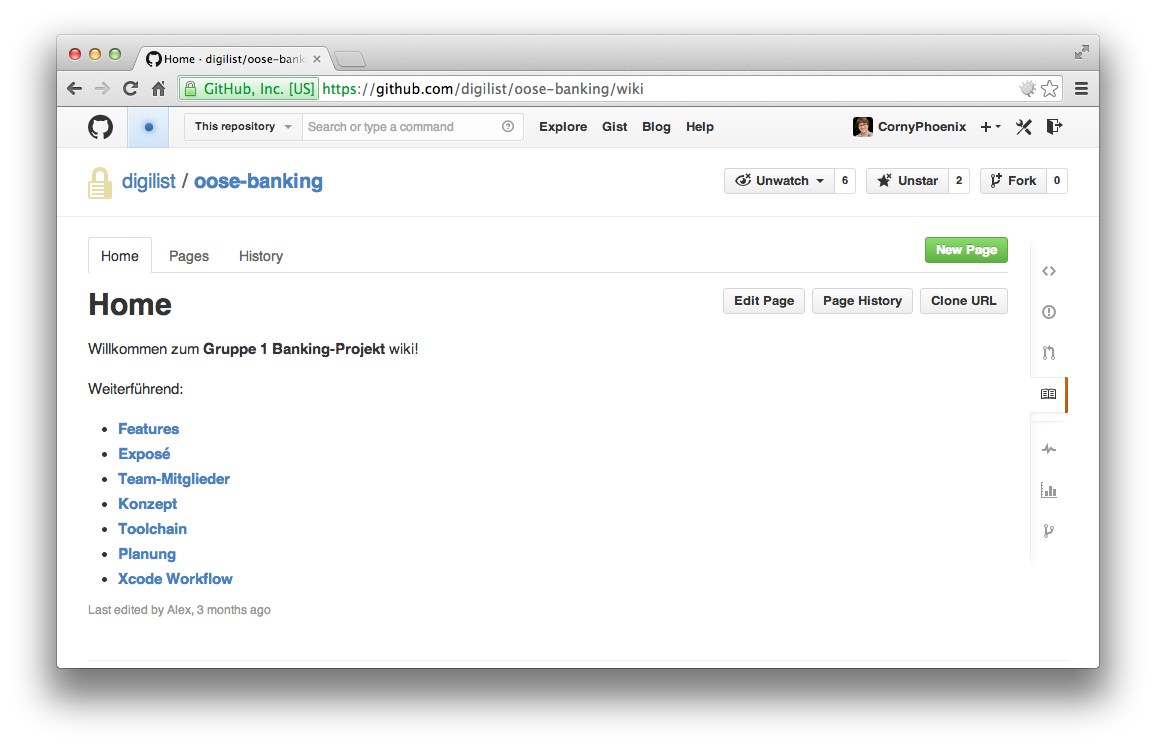
\includegraphics[scale=.3]{Pictures/GitHubWiki}
	\label{fig:GitHubWiki}
	\caption{GitHub-Wiki für den Wissensaustausch}
\end{figure}
\subsection{Konzept und erster Entwurf}
Balsamiq
\begin{figure}
	\centering
	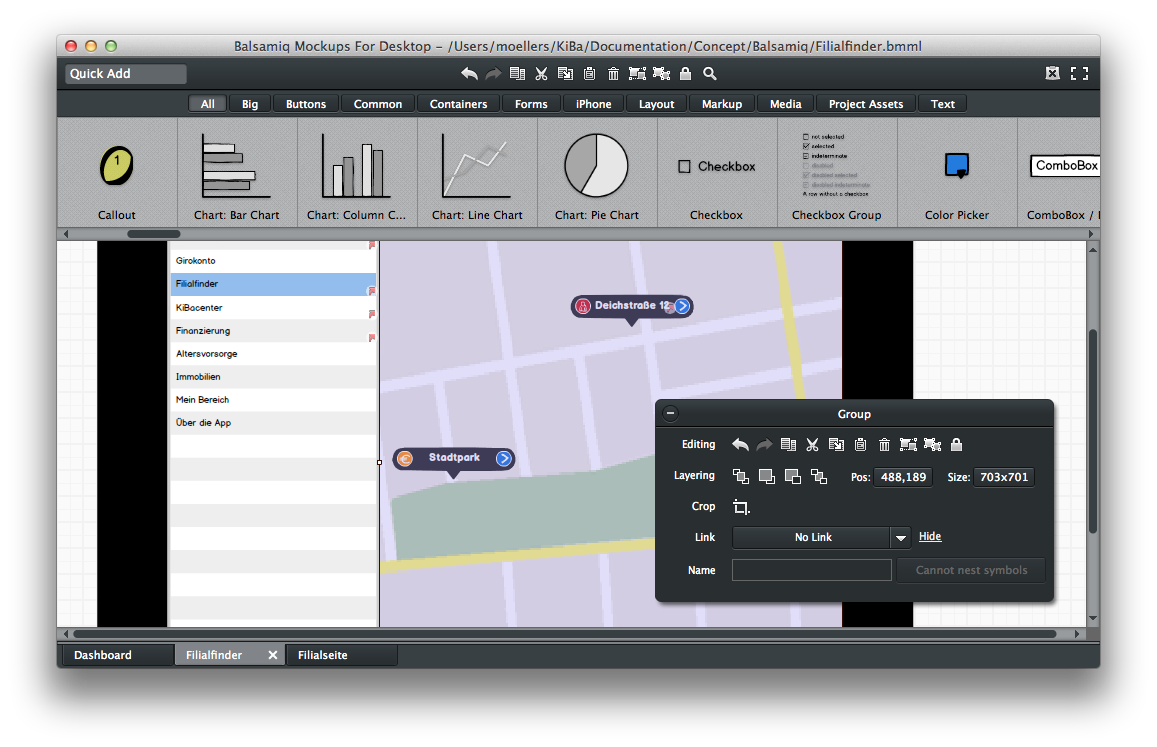
\includegraphics[scale=.3]{Pictures/BalsamiqEntwurf}
	\label{fig:BalsamiqEntwurf}
	\caption{Entwerfen mit Balsamiq}
\end{figure}
\subsection{Design- und Textsatztools}
Lua\LaTeX{}, Adobe Illustrator/Photoshop
\begin{figure}
	\centering
	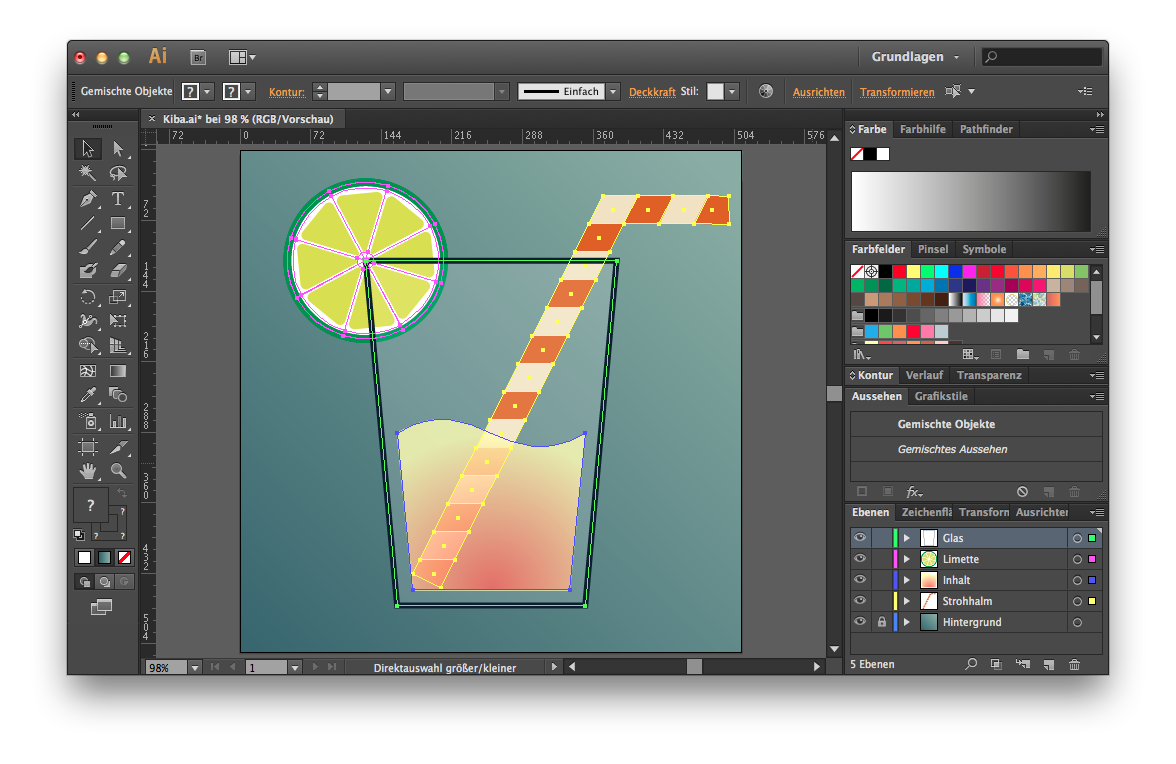
\includegraphics[scale=.3]{Pictures/IllustratorIcon}
	\label{fig:IllustratorIcon}
	\caption{Designen des KiBa-Icons mit Adobe Illustrator}
\end{figure}
\begin{figure}
	\centering
	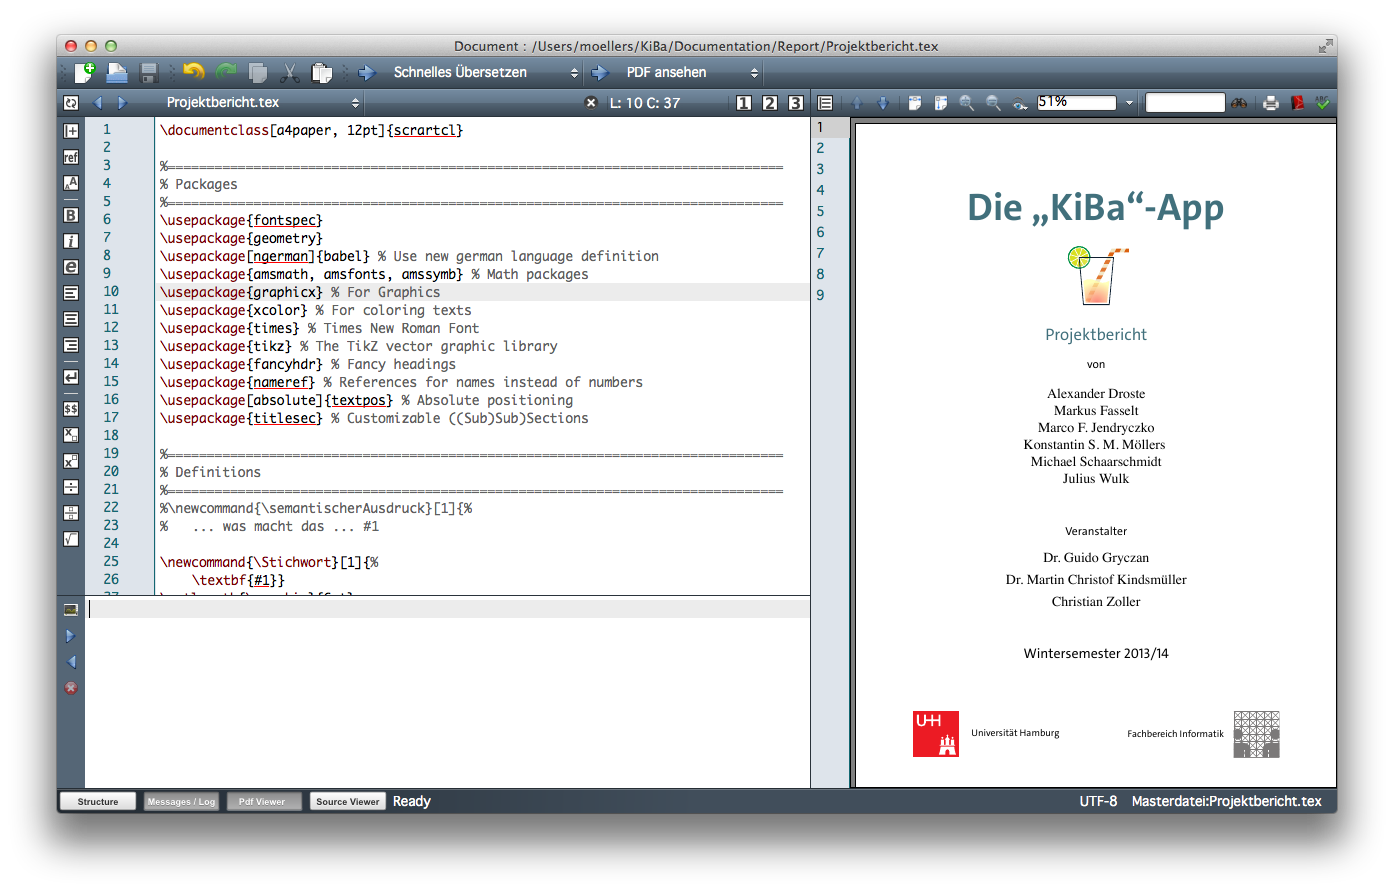
\includegraphics[scale=.3]{Pictures/LaTeXBericht}
	\label{fig:LaTeXBericht}
	\caption{Setzen des Projektberichts mit Lua\LaTeX}
\end{figure}